\subsection{System Integration}

The firmware and hardware were co-designed to ensure seamless integration, with all peripherals and control structures mapped directly to hardware interfaces defined at the PCB design stage. The firmware architecture abstracts low-level hardware interaction through driver modules, allowing the stabilisation logic and control loops to operate independently of specific sensor or motor hardware as long as the communication interface remains consistent.

Integration consisted primarily of flashing the firmware onto the custom PCB and verifying that all I/O mappings aligned with the predefined pin assignments for motors, sensors, and communication interfaces. These pin mappings are fixed in hardware and therefore defined early in the design process to avoid later integration conflicts.

\textbf{Integration Scope}
\begin{itemize}
    \item Flight controller (ESP32) interfaced with IMU, ToF sensor, and motor drivers via I\textsuperscript{2}C, UART, and PWM.
    \item Power distribution validated across battery input, onboard regulators, and USB programming rail.
    \item Mechanical frame provides physical constraints for airflow, sensor line-of-sight, and connector accessibility.
    \item WebSocket communication used to validate telemetry and control signal flow during integration testing.
\end{itemize}

\begin{table}[H]
\centering
\renewcommand{\arraystretch}{1.2}
\begin{tabular}{|p{4cm}|p{9cm}|}
\hline
\rowcolor{gray!15}
\textbf{Subsystem} & \textbf{Integration Checkpoint} \\
\hline
Motor Control & PWM outputs verified against PCB pinout; each channel tested via serial command to confirm expected rotation. \\
\hline
Sensor Interfaces & IMU and ToF sensor initialisation confirmed over I\textsuperscript{2}C with valid data streaming into state estimator. \\
\hline
Power System & USB priority over battery verified; 3.3\,V rail checked under load during active sensor and Wi-Fi transmission. \\
\hline
Communication Link & WebSocket telemetry and setpoint commands validated \\
\hline
Mechanical Fit & PCB alignment, connector access, and sensor line-of-sight confirmed within frame tolerances. \\
\hline
\end{tabular}
\caption{System-Level Integration Verification Points}
\label{tab:system-integration}
\end{table}

\noindent All subsystems were integrated according to version-controlled interface definitions, and validated sequentially through subsystem and combined functional testing. Final system integration is shown in Fig.~\ref{fig:complete-drone}.

\temp{Add completed drone figure}

% \begin{figure}[H]
%     \centering
%     \includegraphics[width=0.7\textwidth]{img/completed-drone.png}
%     \caption{Completed Integrated Drone System}
%     \label{fig:complete-drone}
% \end{figure}

%-------------------------------------------------------------% 
\pagebreak
\subsection{Stakeholder Engagement}
Stakeholder engagement was conducted continuously throughout the project to ensure that client expectations and engineering objectives were aligned. Engagement occurred primarily during the first six weeks (Weeks 1–6), which corresponded to the initial requirements elicitation and design clarification phases. Communication was maintained through information sessions, formal technical query (TQ) submissions, and direct email correspondence with both the client and the unit coordinator.

During the early project stages, stakeholder engagement focused on understanding and refining the drone’s intended capabilities, constraints, and performance criteria. Key outcomes included clarification of power supply specifications, obstacle detection behaviours, and the structure of autonomous flight patterns. 

The process followed an iterative engineering cycle:
\begin{enumerate}
    \item \textbf{Information Sessions:} Weekly sessions with the client to discuss requirements and ask any additional questions.
    \item \textbf{Technical Queries (TQs):} Formal written submissions to document design uncertainties and receive responses.
    \item \textbf{Email Correspondence:} Direct communication used to clarify requirements due to changes in the project scope.
\end{enumerate}

\subsection{Outcomes of Engagement}

A detailed record of all stakeholder interactions, including questions, responses, is given below:

%--------------------------%
\paragraph{\textbf{Client Meetings and Information Sessions}} \leavevmode

\begin{table}[H]
\centering
\caption{Client Expectations - Indoor Surveillance Drone (Week 1)}
\begin{tabular}{|l|p{11cm}|}
\hline
\textbf{Date} & 24/07/2025 (Week 1) \\ \hline
\textbf{Information Session Item} & \textbf{Notes} \\ \hline
1 & Open-source software must be used. \\ \hline
2 & Client requirements may be negotiated with the client. \\ \hline
\end{tabular}
\end{table}

\begin{table}[H]
\centering
\caption{Technical Queries and Client Responses (Weeks 2-5)}
\begin{tabular}{|p{3cm}|p{8cm}|p{3.5cm}|}
\hline
\textbf{Date} & \textbf{Query / Response Summary} & \textbf{Notes / Priority} \\ \hline
31/07/2025 (W2) & \textbf{TQ1:} Desired drone behaviour upon obstacle detection (stop, reverse, turn). & Medium \\ \hline
 & \textbf{Client Response:} Stop and hover; shutdown if obstruction persists. & \\ \hline
31/07/2025 (W2) & \textbf{TQ2:} Requirement for drone movement patterns—preprogrammed or flexible. & High \\ \hline
 & \textbf{Client Response:} Preprogrammed patterns to be given 1-2 weeks before demo; simple polygon-based patterns required. & Plan flexible design early. \\ \hline
07/08/2025 (W3) & \textbf{TQ3:} Battery configuration—two 1S or one 2S acceptable? & Medium \\ \hline
 & \textbf{Client Response:} Only one battery allowed (< 800mAh). & \\ \hline
15/08/2025 (W4) & No technical queries this week. & -- \\ \hline
23/08/2025 (W5) & \textbf{TQ4:} Use of breakout board for IR sensor (VL53L0X). & Medium \\ \hline
 & \textbf{Client Response:} Approved. &  \\ \hline
23/08/2025 (W5) & \textbf{TQ5:} Permission to mark start position with coloured/reflective tape. & Low \\ \hline
 & \textbf{Client Response:} Approved. & \\ \hline
\end{tabular}
\end{table}

\begin{table}[H]
\centering
\caption{Additional Information and Constraints}
\begin{tabular}{|p{0.5cm}|p{13cm}|}
\hline
 & \textbf{Client Notes} \\ \hline
1 & Drifting should be below 10 cm before stabilisation. \\ \hline
2 & Object detection is for non-transparent objects only. \\ \hline
3 & Surveillance camera must record video and optionally allow hover height adjustment. \\ \hline
4 & ESCs must be part of the PCB. \\ \hline
5 & Final testing location: MATH151. \\ \hline
6 & Clarified that focus is on drone performance, not camera hardware. \\ \hline
\end{tabular}
\end{table}

%--------------------------%
\paragraph{\textbf{Requirement Changes}} \leavevmode

During Week 6, the project team and client reviewed and refined the ranked and additional requirements.  The proposed changes involved removing requirements that were no longer feasible given the reduced project capacity and the updated system scope, as the number of members had reduced significantly. This was from six members initially to four by August 1, and two by August 25. No new requirements were added; instead, the scope was greatly reduced. The description of these changes can be found in Appendix~\ref{app:req-changes}.

%--------------------------%
\pagebreak
\paragraph{\textbf{Stakeholder Engagement Summary:}} \leavevmode

Through structured communication, the team achieved the following: \

\begin{tabular}{|p{4cm}|p{10cm}|}
\hline
\rowcolor{gray!15}
\textbf{Activity} & \textbf{Outcome / Actions Closed} \\
\hline
Initial Client Information Sessions (Weeks 1–2) & Defined project expectations and clarified client preferences. Confirmed use of open-source software and flexibility for negotiating requirements. \\ \hline
Technical Query Submissions (Weeks 2–5) & Established operational behaviours for obstacle detection and response (stop, hover, or shutdown). Confirmed flexibility for flight paths with both predefined and custom polygonal trajectories. \\ \hline
Hardware Clarifications & Defined hardware constraints including the use of a single battery (<800mAh), integrated PCB with ESCs, and allowance for breakout components (e.g., IR sensor). \\ \hline
Requirement Tracking and Documentation & Logged all communications and technical clarifications in a shared document. Updated requirements list to reflect client feedback and design feasibility. \\ \hline
Week 6 Client Meeting – Requirement Review & Reviewed all ranked and additional requirements to align project scope with reduced team capacity. Prioritised core functionalities such as flight stability, safety, and manual override. \\ \hline
Requirement Rationalisation & Removed redundant or infeasible requirements (e.g., complex autonomous navigation and multi-pattern path options). Ensured compliance with budget and technical constraints. \\ \hline
Final Client Approval & Confirmed revised and re-ranked requirements list with the client. Finalised scope for design and testing phases based on approved specification. \\ \hline
\end{tabular}

%-------------------------------------------------------------% 
\pagebreak
\subsection{Safety Issues}
This safety plan applies to bench electronics work, soldering and rework, and controlled indoor hover testing. All activities are conducted in designated laboratory spaces with restricted access during active testing. Risk ratings follow a consequence–likelihood–exposure (C×L×E) model. Mitigations apply the hierarchy of hazard control: elimination, substitution, e
ngineering control, administrative control, and PPE as a final layer. Full details are contained in the risk register.

\vspace{0.5em}
\textbf{Operational Boundaries and Controls:}

\begin{tabular}{|p{4cm}|p{11.5cm}|}
\hline
\rowcolor{gray!15}\textbf{Aspect} & \textbf{Defined Limits and Requirements} \\ \hline
Environment & Indoor test room only; access restricted during hover tests with signage placed outside. \\ \hline
Training & All personnel must complete soldering and Li-Po handling inductions before handling any equipment. \\ \hline
Hover Testing & Hover altitude limited to 1.25\,m AGL; any adjustment beyond this permitted only during setup phases with props disarmed. \\ \hline
Battery Management & Only 1S/2S Li-Po <800\,mAh packs approved; no swollen or damaged cells. Charging supervised with fire blanket or sand bucket available. \\ \hline
Personnel & Minimum two people: Test Lead with authority to abort and Spotter monitoring environmental conditions and escape paths. \\ \hline
PPE & Safety glasses and closed footwear mandatory at all times; nitrile gloves required for chemical or flux handling tasks. \\ \hline
\end{tabular}

\vspace{0.5em}
\textbf{Acceptance Criteria:} All tests must demonstrate thermal compliance, fail-safe functionality, clean electrical behaviour, and incident-free operation. Logs and checklists must be completed to satisfy traceability requirements.

The following table summarises key hazards, their associated risks, and control approaches.

\begin{tabular}{|p{2.3cm}|p{4.5cm}|p{4cm}|p{3.8cm}|}
\hline
\rowcolor{gray!15}\textbf{Hazard} & \textbf{Risks/Mechanism} & \textbf{Controls Implemented} & \textbf{Procedure} \\ \hline
Heating & Localised MOSFET heating or soldering burns & Copper pours, current limiting, heat mats & IR checks, switch-off when idle \\ \hline
Cuts/Abrasions & Propeller lacerations or tool injuries & Shrouds, guarded tools, PPE & Bench test first, enable arming LED cues \\ \hline
Sparking & Short circuits or solder bridging & Heat-shrink, clearance design & continuity test, no live soldering \\ \hline
Battery & Thermal runaway or over-discharge & Voltage alarms, visual inspection & Remove damaged cells, fire control kit on-site \\ \hline
Trips/Spills & Loose cables/liquids in walkways & Cable trays, dry floor policy & End-of-session clearance audit \\ \hline
Collisions & Impact during hover test & Altitude limit, prop shields & Incident log, abort protocol \\ \hline
Fumes & Flux fumes, UFPs from printing & Extraction fans, gloves & Ventilation check, SDS access \\ \hline
\end{tabular}

%-------------------------------------------------------------% 
\pagebreak
\subsection{Ethical Issues}
Testing takes place in a shared laboratory environment, so ethical considerations focus on safety, responsible data handling, and clear usage boundaries for open-source release. Exclusion zones will be clearly marked, and written approval is obtained from space owners before any powered testing. A spotter is always present to ensure that no unauthorised person enters the test area.

\vspace{0.5em}
\textbf{Data and Recording:}  
The onboard camera remains disabled by default and is only activated during scheduled and approved hover trials. Any footage containing identifiable individuals will require written consent before capture. Recordings, if taken, are stored in encrypted form, retained for no longer than seven days and permanently deleted upon request.

\vspace{0.5em}
\textbf{Wireless Communication:}  
Wi-Fi telemetry operates under least-privilege access principles. No personal device identifiers are logged. RF transmissions remain within laboratory and local regulatory limits. Channels that may conflict with co-located research equipment are excluded.

\vspace{0.5em}
\textbf{Open-Source Release and Responsible Use:}  
All CAD, firmware, and PCB files will be published under a permissive open-source license. Documentation will clearly state:

\begin{itemize}
    \item Intended operation is indoor hover testing only, with shrouded rotors and fully functional fail-safes.
    \item Prohibited uses include surveillance without explicit consent, public outdoor operation, weaponisation, or disabling of safety systems.
    \item Recommended safe substitution components, correct Li-Po disposal procedures, and repair instructions using reprintable PETG parts.
\end{itemize}

This ensures that any derivative builds acknowledge ethical and safety boundaries aligned with the project's academic intent.

%-------------------------------------------------------------% 
\pagebreak
\subsection{Top 5 Risks and Mitigations}

The following risks have the highest inherent risk ranking based on (C×L×E). Mitigations follow the hierarchy of controls, and each risk includes a defined verification test to confirm that controls are effective.

\textbf{RISK-01: Slips \& Trips}

\begin{tabular}{@{}p{3cm}p{13cm}@{}}
\toprule
\textbf{Inherent Risk} & 1500 (Very High) \\
\textbf{Key Causes} & Loose cables, tools obstructing walkways, congested bench area. \\
\textbf{Mitigations} &
• \textbf{Elimination:} Keep walkways clear, remove floor clutter. \newline
• \textbf{Engineering:} Use cable trays, tape down leads. \newline
• \textbf{Administrative:} End-of-session clearance checks, clear-aisle policy. \newline
• \textbf{PPE:} Closed-toe shoes. \\
\textbf{Verification Test} & Walkway audit: zero loose cables/tools; aisles $\geq$900\,mm clear. Pass, no hazards found \\
\textbf{Residual Risk} & Low \\
\bottomrule
\end{tabular}
\vspace{0.6em}

\textbf{RISK-02: Poor Ventilation / Asphyxiation}

\begin{tabular}{@{}p{3cm}p{13cm}@{}}
\toprule
\textbf{Inherent Risk} & 750 (Very High) \\
\textbf{Key Causes} & Soldering without fume extraction; extended work in enclosed areas. \\
\textbf{Mitigations} &
• \textbf{Substitution:} Use low-odour, rosin-free flux. \newline
• \textbf{Engineering:} Enable local fume extraction with filters. \newline
• \textbf{Administrative:} Ventilation checks before work, time limits on solder tasks. \newline
• \textbf{PPE:} Optional respirator if extraction unavailable. \\
\textbf{Verification Test} & Fume extractor active, filter in place, ventilation checklist signed. Pass, all conditions met \\
\textbf{Residual Risk} & Low \\
\bottomrule
\end{tabular}
\vspace{0.6em}

\textbf{RISK-03: Cuts / Abrasions}

\begin{tabular}{@{}p{3cm}p{13cm}@{}}
\toprule
\textbf{Inherent Risk} & 450 (High) \\
\textbf{Key Causes} & Sharp tools or part edges, damaged 3D prints or PCBs. \\
\textbf{Mitigations} &
• \textbf{Elimination:} Deburr and smooth printed/metal edges. \newline
• \textbf{Engineering:} Use tool guards and retractable blades. \newline
• \textbf{Administrative:} Tool-use training and blade return protocol. \newline
• \textbf{PPE:} Safety glasses; cut-resistant gloves if needed. \\
\textbf{Verification Test} & All sharp edges smoothed; blades stored safely; PPE worn during cutting. Pass, all conditions met \\
\textbf{Residual Risk} & Low \\
\bottomrule
\end{tabular}
\vspace{0.6em}

\pagebreak
\textbf{RISK-04: Burns (Soldering / Hot Components)}

\begin{tabular}{@{}p{3cm}p{13cm}@{}}
\toprule
\textbf{Inherent Risk} & 450 (High) \\
\textbf{Key Causes} & Contact with hot soldering iron tips or overheated MOSFETs. \\
\textbf{Mitigations} &
• \textbf{Engineering:} Use tip stands and heat-proof mats. \newline
• \textbf{Administrative:} Do not leave powered irons unattended. \newline
• \textbf{PPE:} Safety glasses; heat-resistant gloves if required. \\
\textbf{Verification Test} & Iron stored in stand; heat mat in use; motor driver $<85^\circ$C after 5\,min hover. Pass, all conditions true \\
\textbf{Residual Risk} & Low \\
\bottomrule
\end{tabular}
\vspace{0.6em}

\textbf{RISK-05: Emissions (Solder / 3D-Print Fumes)}

\begin{tabular}{@{}p{3cm}p{13cm}@{}}
\toprule
\textbf{Inherent Risk} & 270 (Medium) \\
\textbf{Key Causes} & Flux fumes, ultrafine particle emissions from filament heating. \\
\textbf{Mitigations} &
• \textbf{Substitution:} Lead-free solder and low-emission filament. \newline
• \textbf{Engineering:} Local fume extraction for soldering and printing. \newline
• \textbf{Administrative:} Store chemicals sealed; SDS available. \newline
• \textbf{PPE:} Safety glasses; nitrile gloves for solvent handling. \\
\textbf{Verification Test} & Extraction active and SDS visible; PPE worn when handling resin/solvents. Pass, all conditions true \\
\textbf{Residual Risk} & Low \\
\bottomrule
\end{tabular}

%-------------------------------------------------------------% 
\pagebreak
\subsection{Process of Assembly}

\begin{table}[H]
\centering
\renewcommand{\arraystretch}{1.3}
\begin{tabular}{|p{4cm}|p{10cm}|}
\hline
\rowcolor{gray!15}
\textbf{Step} & \textbf{Action / Details} \\
\hline
\rowcolor{gray!5}
\multicolumn{2}{|c|}{\textbf{PCB Bring-Up}} \\
\hline
Unbox PCB & Inspect for solder mask defects, visual solder bridges, and damaged pads. \\
\hline
Continuity Test & 1) VBAT to GND (no short)  \newline 2) 3V3 to GND (no short)  \newline 3) Key nets per schematic. \\
\hline
ESD Protection & Use ESD mat and strap before populating components. \\
\hline
Populate Components & 1) 10 µF capacitor  \newline 2) 100 nF capacitor  \newline 3) ESP32 module  \newline 4) Female header pins: bent pins outwards for front sensor, vertical pins downward for bottom sensor. \\
\hline
Post-Solder Check & Perform continuity test on soldered components. \\
\hline
Voltage Rails & Verify 3V3 = 3.3 V. \\
\hline
Temperature Check & Ensure no component is abnormally hot at idle. \\
\hline
\rowcolor{gray!5}
\multicolumn{2}{|c|}{\textbf{3D-Printed Frame Assembly}} \\
\hline
Print Frame & 1) Material: PETG  \newline 2) Supports: tree  \newline 3) Infill: ~7\% gyroid  \newline 4) Wall thickness: 2 perimeters. \\
\hline
Post-Processing & 1) Remove supports and smooth edges; inspect for defects  \newline 2) Open front of frame for PCB insertion  \newline 3) Ensure no component contacts 3D printed surfaces; PCB sits flush  \newline 4) Slide motors into friction-fit holders. \\
\hline
Check Fit & 1) PCB flat  \newline 2) Connectors accessible  \newline 3) No compression on ESP32  \newline 4) Edges flush. \\
\hline
\rowcolor{gray!5}
\multicolumn{2}{|c|}{\textbf{Modular Options Assembly}} \\
\hline
Battery Cage & 1) Optionally insert under main frame. \\
\hline
Camera Module Holder & 1) Optionally attach on top of main frame. \\
\hline
Leg Pieces & 1) Insert into designated holes under main frame. \\
\hline
\rowcolor{gray!5}
\multicolumn{2}{|c|}{\textbf{Pre-Run Checks}} \\
\hline
Lead Routing & 1) Route motor/JST leads away from rotor sweep  \newline 2) Secure with tie-downs. \\
\hline
Clearance Check & 1) Ensure full clearance with guards  \newline 2) No wire chafe  \newline 3) Connectors latched  \newline 4) Motors held firmly. \\
\hline
Mechanical Tests & 1) Run shake or stability tests \textit{[location TBD]}. \\
\hline
Firmware Test & 1) Power on without propellers  \newline 2) Confirm ESP32 boots, sensors initialise  \newline 3) Each motor spins once  \newline 4) Verify serial output, LED states correct. \\
\hline
\end{tabular}
\caption{ESP Assembly and Pre-Run Procedure}
\label{tab:esp-assembly-numbered}
\end{table}

\textbf{Soldering Guide} \\
The following steps illustrate the initial PCB soldering process, showing component placement and orientation.

\begin{figure}[H]
    \centering
    \begin{subfigure}[b]{0.4\textwidth}
        \centering
        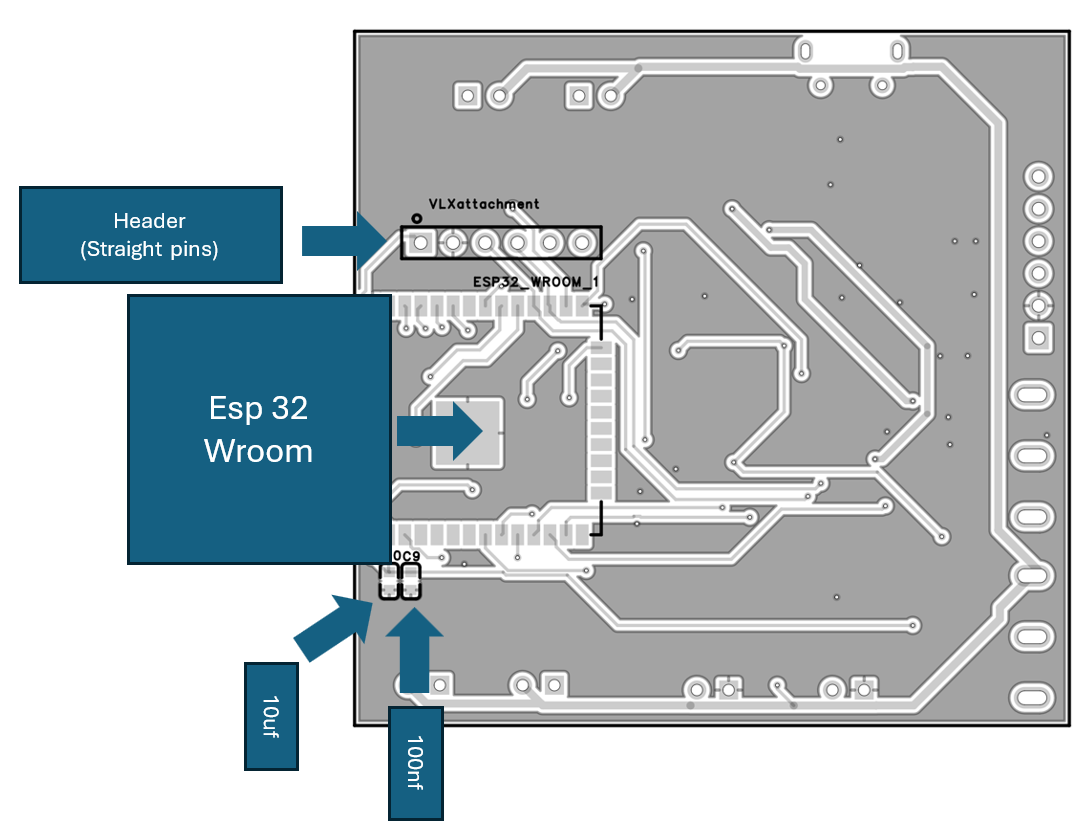
\includegraphics[width=\textwidth]{img/assembly-1.png}
        \caption{Step 1}
    \end{subfigure}
    \hfill
    \begin{subfigure}[b]{0.4\textwidth}
        \centering
        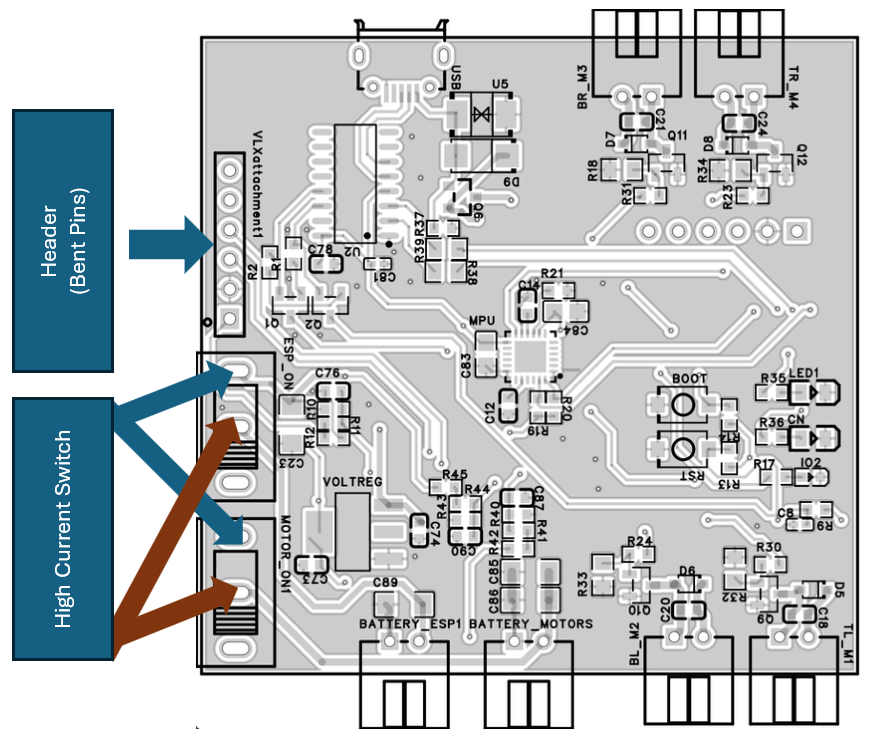
\includegraphics[width=\textwidth]{img/assembly-2.png}
        \caption{Step 2}
    \end{subfigure}
    \caption{ESP Assembly Steps}
\end{figure}

\textbf{Main Frame} \\
This image shows the 3D-printed main frame of the drone, which provides structural support for the PCB, motors, and any modular components.

\begin{figure}[H]
    \centering
    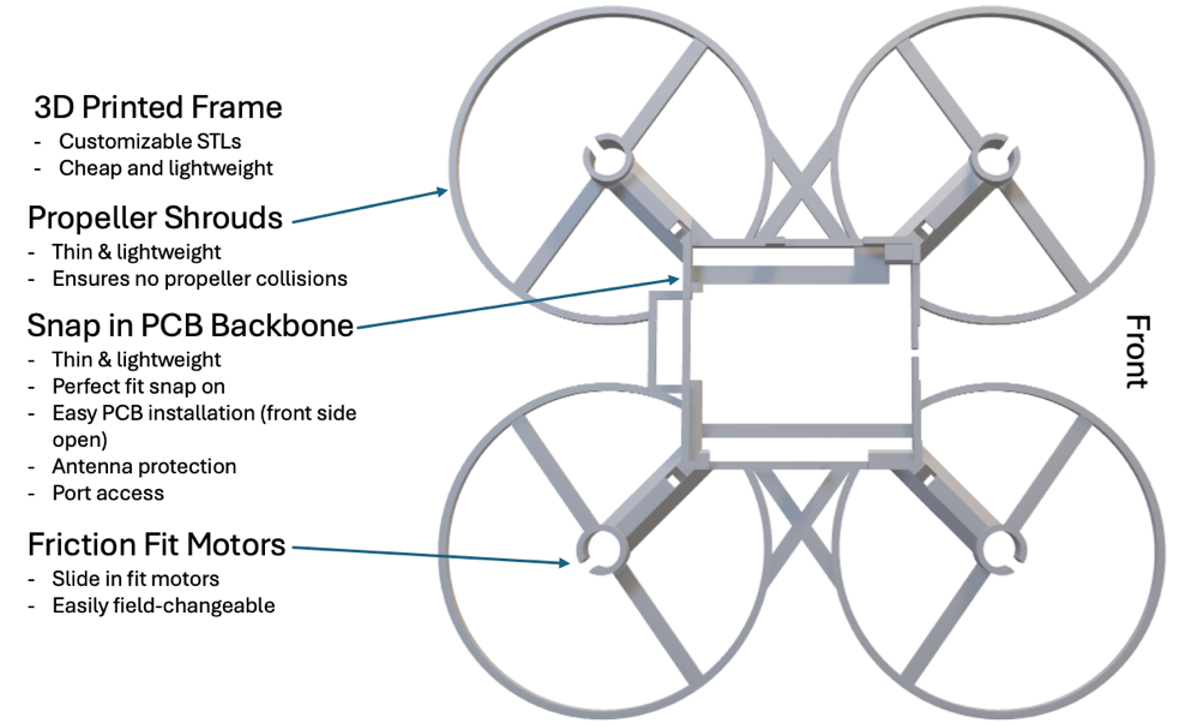
\includegraphics[width=0.8\textwidth]{img/assembly-3.png}
\end{figure}

\pagebreak
\textbf{Frame Additions} \\
These figures illustrate optional components being inserted into the main frame, such as the camera holder and legs and can be removed, changed and altered easily to fit with the main frame.

% \begin{figure}[H]
%     \centering
%     \begin{subfigure}[b]{0.48\textwidth}
%         \centering
%         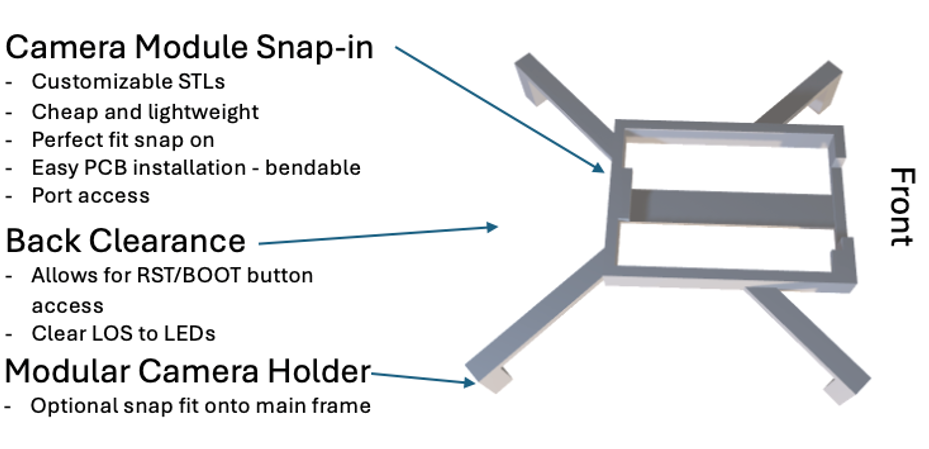
\includegraphics[width=\textwidth]{img/assembly-4.png}
%         \caption{Step 1}
%         \label{fig:assembly-4}
%     \end{subfigure}
%     \hfill
%     \begin{subfigure}[b]{0.48\textwidth}
%         \centering
%         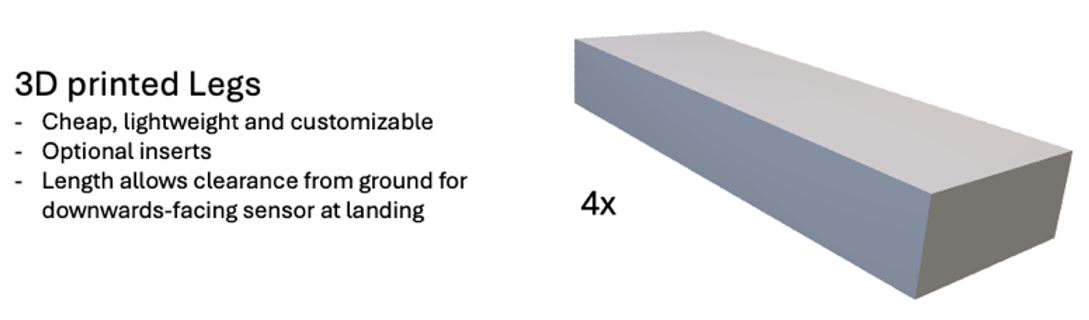
\includegraphics[width=\textwidth]{img/assembly-5.png}
%         \caption{Step 2}
%         \label{fig:assembly-5}
%     \end{subfigure}
%     \caption{ESP Assembly Steps}
%     \label{fig:extras-assembly-steps}
% \end{figure}

\begin{figure}[H]
    \centering
    \begin{subfigure}[b]{0.3\textwidth}
        \centering
        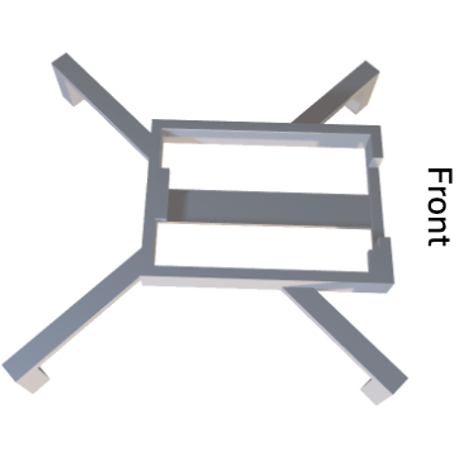
\includegraphics[width=\textwidth]{img/assembly-4b.png}
        \caption{Camera Mount}
    \end{subfigure}
    \vspace{0.5cm}
    \begin{subfigure}[b]{0.3\textwidth}
        \centering
        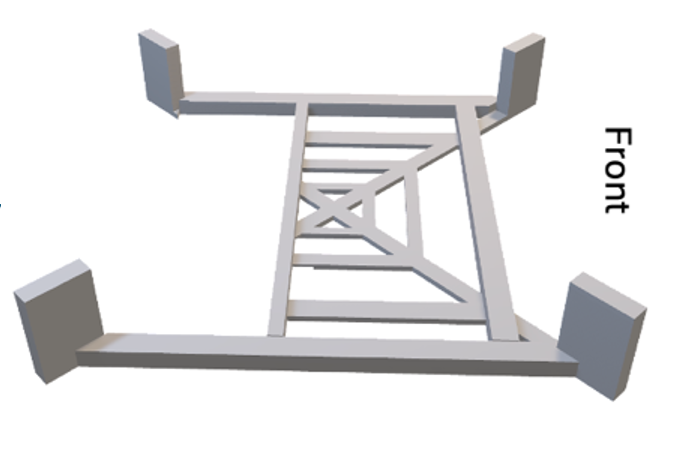
\includegraphics[width=\textwidth]{img/assembly-9b.png}
        \caption{Battery Holder}
    \end{subfigure}
    \vspace{0.5cm} 
    \begin{subfigure}[b]{0.25\textwidth}
        \centering
        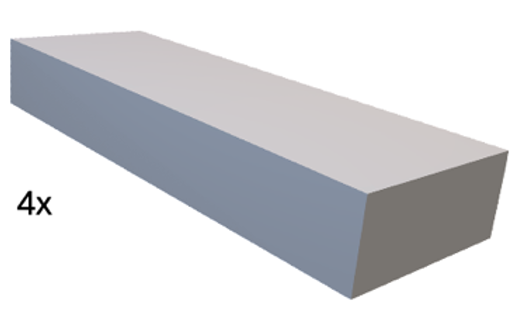
\includegraphics[width=\textwidth]{img/assembly-5b.png}
        \caption{Drone Foot}
    \end{subfigure}
    \caption{Frame Assembly Process}
\end{figure}

% \begin{figure}[H]
%     \centering
%     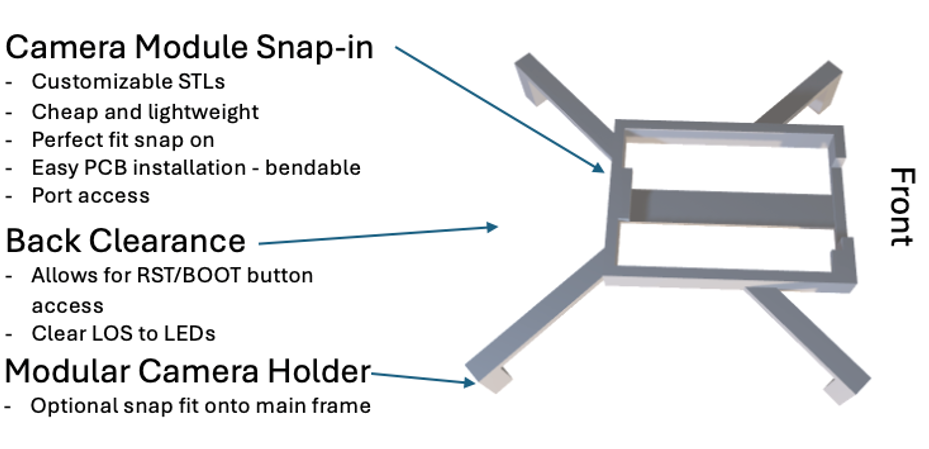
\includegraphics[width=0.6\textwidth]{img/assembly-4.png}
% \end{figure}

% \begin{figure}[H]
%     \centering
%     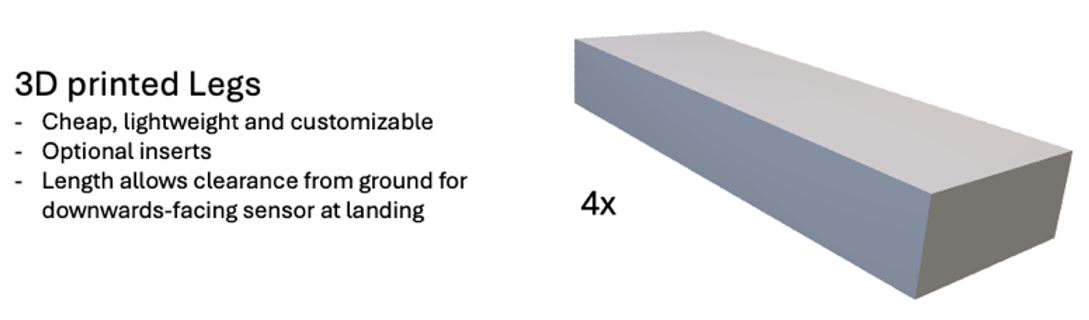
\includegraphics[width=0.6\textwidth]{img/assembly-5.png}
% \end{figure}

% \begin{figure}[H]
%     \centering
%     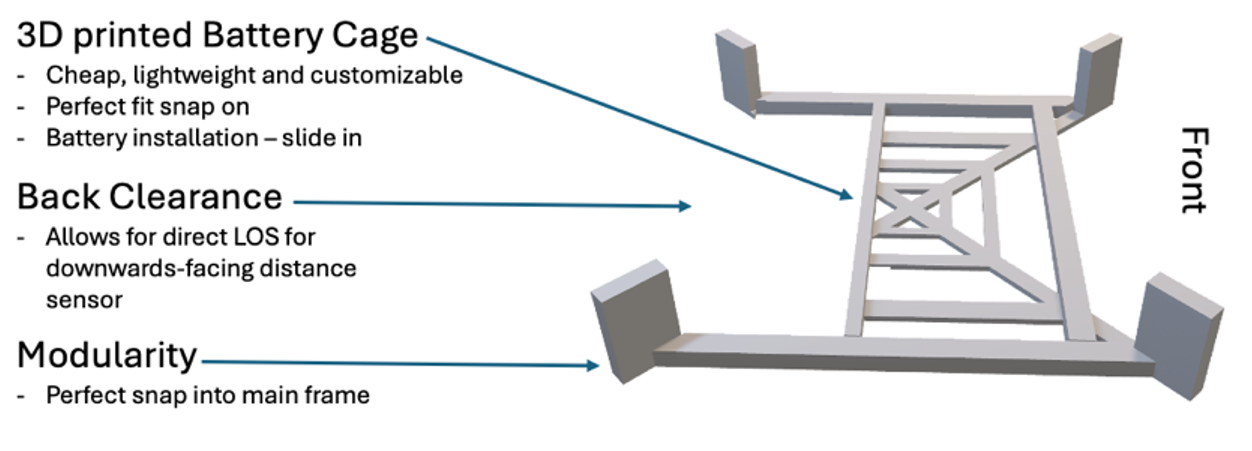
\includegraphics[width=0.6\textwidth]{img/assembly-9.png}
% \end{figure}

% \pagebreak
\textbf{Frame Assembly} \\
The following figures demonstate how the additional frame components can be added to the main frame.

\begin{figure}[H]
    \centering
    \begin{subfigure}[b]{0.45\textwidth}
        \centering
        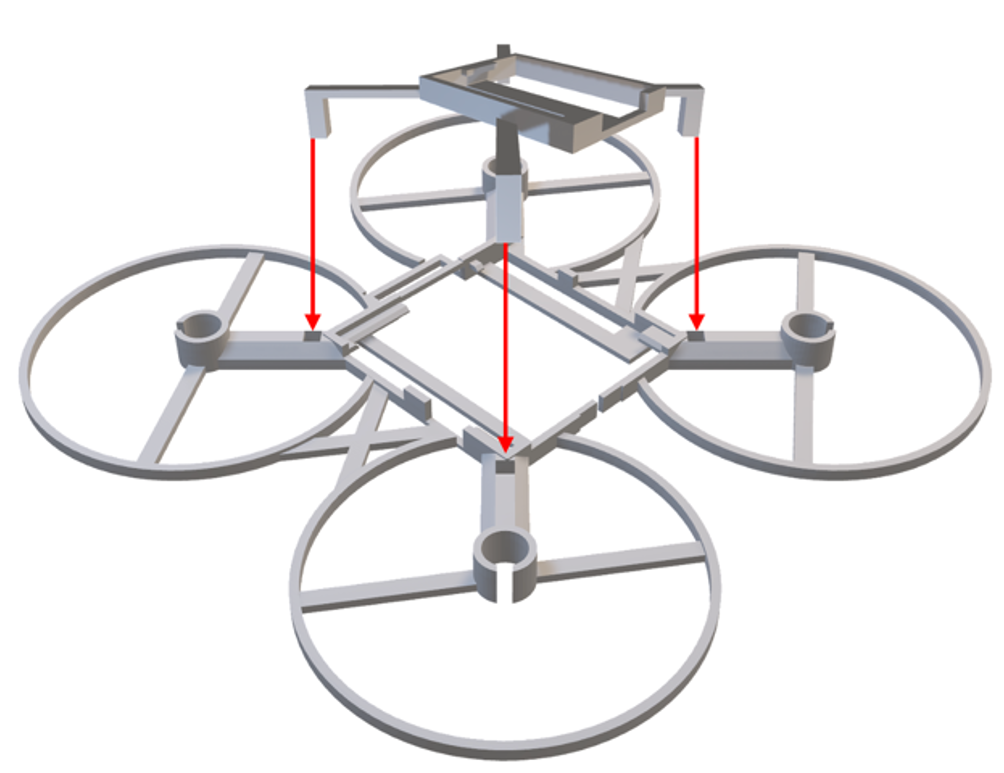
\includegraphics[width=\textwidth]{img/assembly-6.png}
        \caption{Camera Mount}
    \end{subfigure}
    % \vspace{0.5cm} 
    \begin{subfigure}[b]{0.35\textwidth}
        \centering
        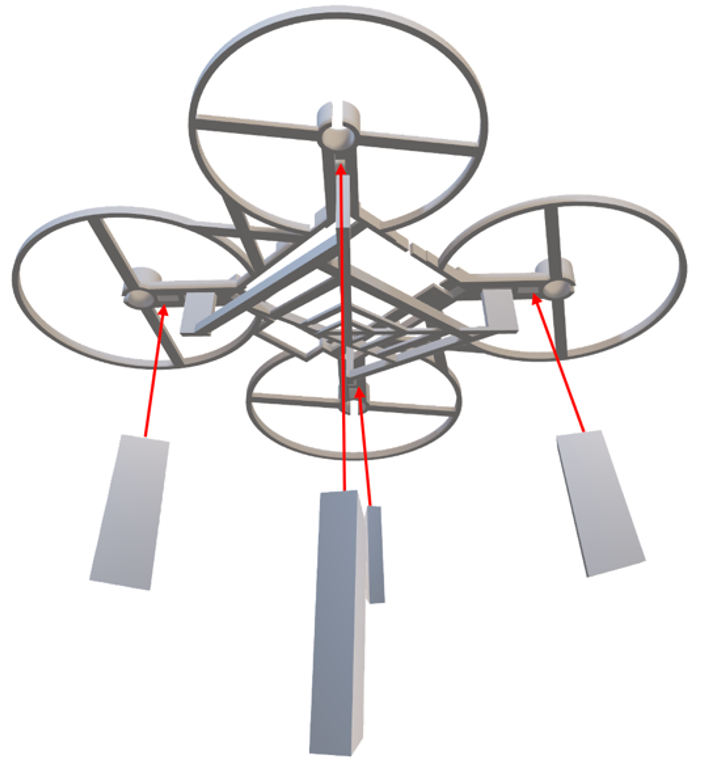
\includegraphics[width=\textwidth]{img/assembly-7.png}
        \caption{Drone Foot}
    \end{subfigure}
    % \vspace{0.5cm}
    \begin{subfigure}[b]{0.35\textwidth}
        \centering
        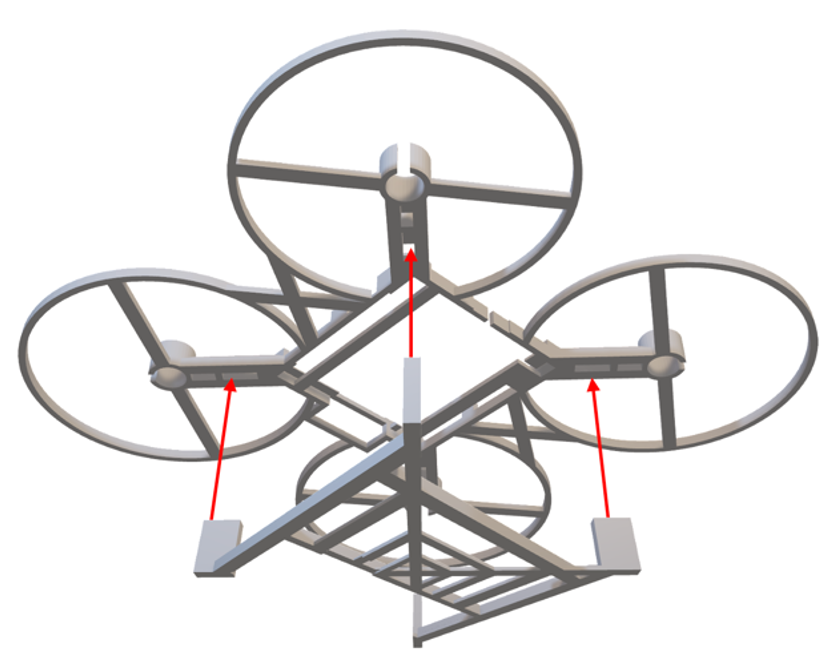
\includegraphics[width=\textwidth]{img/assembly-8.png}
        \caption{Battery Holder}
    \end{subfigure}
    \caption{Frame Assembly Process}
\end{figure}

\pagebreak
A summary of the additions is given below in Table~\ref{tab:frame-add-summary}.

\begin{table}[H]
\centering
\begin{tabular}{|p{3cm}|p{11cm}|}
\hline
\textbf{Module} & \textbf{Features} \\
\hline
Camera Module Snap-In &
o Customizable 3D-printed STL files for design adjustments \newline
o Lightweight and cost-effective \newline
o Perfect snap fit onto main frame \newline
o Easy PCB installation; bendable as needed \newline
o Provides access to ports/connectors \newline
o Back clearance for RST/BOOT buttons and status LEDs \newline
o Optional snap-on camera holder for modularity \\
\hline
3D-Printed Battery Holder & 
o Lightweight, customizable, affordable \newline
o Snap-fit onto main frame \newline
o Easy battery installation \newline
o Back clearance for downward-facing distance sensor \newline
o Supports modular quick insertion/removal \\
\hline
3D-Printed Legs / Drone Feet & 
o Cheap, lightweight, customizable \newline
o Optional inserts for flexible landing configuration \newline
o Sufficient leg length for sensor clearance \newline
o Four legs improve frame stability \\
\hline
\end{tabular}
\caption{Summary of Modular Frame Additions}
\label{tab:frame-add-summary}
\end{table}

%-------------------------------------------------------------% 
\subsection{Design Outputs}
\textbf{Stored at:} \url{https://github.com/koshchey/design-project-flight-controller}

\textbf{Repository Contents:}
\begin{itemize}
    \item \texttt{ELEC5552\_FinalReport\_Team0.pdf}: This report.
    \item \texttt{Final\_Report\_LaTeX/}: Contains all \LaTeX{} source files.
    \item \texttt{Firmware/}: Flight controller firmware (\gls{esp-idf} project).
    \item \temp{To-add}
\end{itemize}

%-------------------------------------------------------------% 
\subsection{Final Costs}
